\section{Compacité}
\begin{definition}
    Soit $F \subset E$. Un \textbf{recouvrement ouvert} de $F$, est une union des enesembles ouverts:  $\bigcup_{i \in I} U_i$ tel que $F \subset \bigcup_{i \in I} U_i$
\end{definition}
\begin{eg}
    Soit $F = ]0, 1[$. Soit $A = \left\{]\frac{1}{n}, 1 + \frac{1}{n}[, n \in N\right\}$. $F \subset \bigcup_{n \in N^{*}} A_n$ i.e union infinie des $A_i$ couvre $F$.
\end{eg}
\begin{definition}
    Un ensemble $F \subset E$ est \textbf{compact} si \underline{pour tout} recouvrement ouvert, i.e \underline{pour tout} union des ensembles ouvert $\bigcup_{i \in I} U_i$ qui couvre $F$, on peut prendre un nombre \underline{fini} des  $U_i$ et couvrir $F$.
\end{definition}
\begin{theorem}
    Un ensemble $K \subset E$ est compact, si toute suite $(x_n)_{n \in \N}$ des éléments de $K$, possede une sous-suite qui converge  vers un éléments $x \in K$.
\end{theorem}
\begin{intuition}
    S'il existe tel suite $(x_n)_{n \in \N}$ sans sous-suite convergente vers un éléments de  $K$, donc les valeurs sont en-dehors de  $K$ et donc il existe un ensemble qui couvre $K$  seulement avec un nombre infini des ensembles. 
\end{intuition}
Pourquoi a-t-on besoin de compacité? Car cela nous donne une
\begin{prop}
    \begin{itemize}
        \item Si $K \subset E$ est compact, alors $K$ est fermé et borné.
        \item Si $K$ est compact et  $F$ est fermé, donc  $K \cap F$ est compact. Autrement dire, si $K$ est compact, alors tout fermé $F \subset K$ est compact.
        \item Si $K$ est compact, donc  $K$ est complet.
    \end{itemize}
\end{prop}
\begin{property}
    La différence entre \textit{compacité} et {complecité}:
    \begin{itemize}
        \item complecité nous assure qu'il n'y a pas de trou dans un espace
        \item compacité nous assure qu'un ensemble est fermé et borné
    \end{itemize}
\end{property}
\section{Limites et applications continues}
\begin{definition}
    Soit $(E_{1}, d_1)$ et $(E_2, d_2)$ deux éspaces métriques, $x_0 \in E_1$, $l \in E_2$ et $F: E_1 \to E_2$ une application.
    \begin{enumerate}
        \item On dit que $\lim_{x \to x_0} F(x) = l$ si pour tout $\epsilon > 0, \, \exists \alpha > 0$ tel que pour tout $x \in E_1$ tel que  $d_1(x_0, x) \le \alpha$ on a $d_2(f(x), l) \le \epsilon$ 
        \item On dit que $F$ est continue en  $x_0$ si $\lim_{x \to x_0} f(x) = f(x_0)$
        \item On dit que $F$ est continue si  $F$ est continue en tout $x \in E_1$
    \end{enumerate}
\end{definition}
\begin{prop}\label{def:continuite-topologique}
    definition de la continuité topologique.
    \par
    Soit $(E_{1}, d_1)$ et $(E_2, d_2)$ deux éspaces métriques et la fonction $F: E_1 \to E_2$, on dit que  $F$ est continue si et seulement si:
     \[
         \forall U \subset E_2 \text{ ouvert},  F^{-1}(U) \text{ ouvert}
    \] 
    où $F^{-1}(U) = \{ x \in E_1 \mid F(x) \in U\}$
\begin{figure}[H]
    \centering
    \incfig{continuite-topologique}
    \caption{continuite-topologique}
    \label{fig:continuite-topologique}
\end{figure}
\end{prop}

\begin{preuve} de la proposition-définition \ref{def:continuite-topologique}
   \begin{enumerate}
       \item Montrons que $F$ continue  $\implies$ si $U$ ouvert donc $F^{-1}(U)$ ouvert.
           \par
           Supposons que $F$ continue. Soit  $y \in U$, alors  $\exists x_0 \in F^{-1}(U)$ tel que $F(x_0) = y$, 
           comme  $F$ est continue, donc:  
           \[
               \forall \epsilon > 0, \exists \alpha > 0 \text{ tq } \forall x \in E_1 \text{ tq }  d(x_0, x) < \alpha \implies d(y = F(x_0), x) < \epsilon
           \] 
           Or $U$ est ouvert, alors pour $y$, il existe  $\epsilon$ tq  $B(y, \epsilon) \subset U$, comme $F$ continue, il existe $\alpha$, tq $\forall x \in B(x_0, \alpha), \, y \in B(y, \epsilon) \subset U$. Alors, on a montré que $\forall x \in F^{-1}(U), \, \exists \alpha$ tq $B(x, \alpha) \subset F^{-1}(U)$, donc $F^{-1}(U)$ est ouvert. 
       \item Montrons que $F$ continue  $\impliedby$ si $U$ ouvert donc $F^{-1}(U)$ ouvert.
           Supposons que $\forall U$ ouvert $\subset E_2$, $F^{-1}(U)$ est ouvert. 
           \par
           Soit $y \in U$ et $\epsilon > 0$, posons: $U := B(y, \epsilon)$ ouvert  $\subset E_2$ donc $F^{-1}(U)$ ouvert, d'où $\forall x \in F^{-1}(U) \, \exists \alpha > 0$ tq $B(x, \alpha) \subset F^{-1}(U)$. 
           Par la définition de la boule ouverte, on a:
           \[
               \forall y := f(x_0), \forall \epsilon > 0, \exists \alpha > 0, \forall x \in E_1 \text{ tq } d(x_0, x) < \alpha, d(f(x), y = f(x_0)) < \epsilon
           \] 
   \end{enumerate} 
\end{preuve}
\begin{eg} résultat de cette proposition.
    Prenons la fonction: $f(x) = x^2$.  $f^{-1}(]4, 9[) = \{x \in \R \mid 4 < x^2 < 9\} = ]-3, -2[ \cup ]2, 3[$. Autrement dire, la continuité de $f$ (évident) donne que  $U = ]4, 9[$ ouvert, alors $f^{-1}(U)$ aussi ouvert.
    \begin{figure}[H]
        \centering
        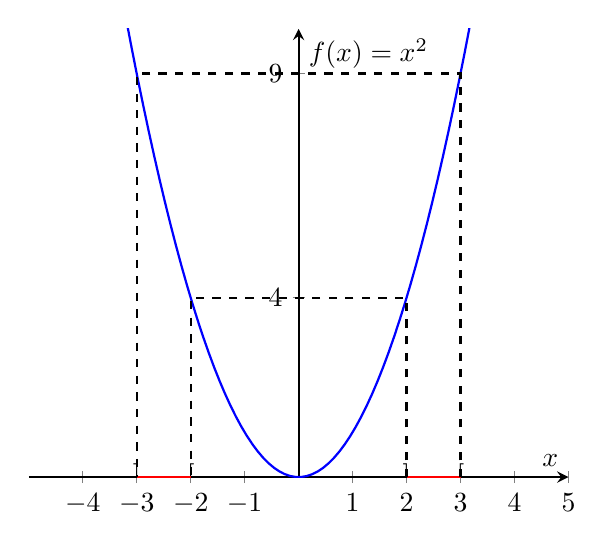
\begin{tikzpicture}
            \begin{axis}[
                axis lines = middle,
                xlabel = $x$,
                ylabel = {$f(x) = x^2$},
                xmin=-5, xmax=5,
                ymin=0, ymax=10,
                samples=100,
                domain=-5:5,
                xtick={-4,-3,-2,-1,0,1,2,3,4,5},  % Custom x-axis numbers
                ytick={0,4,9},   % Custom y-axis numbers
                thick
                ]
                \addplot[blue, thick] {x^2};
                \coordinate (a) at (2, 0);
                \node (_) at (a){$]$};
                \coordinate (b) at (-2, 0);
                \node (_) at (b){$[$};
                \coordinate (c) at (3, 0);
                \node (_) at (c){$[$};
                \coordinate (d) at (-3, 0);
                \node (_) at (d){$]$};

                \coordinate (fa) at (2, 4);
                \coordinate (fb) at (-2, 4);
                \coordinate (fc) at (3, 9);
                \coordinate (fd) at (-3, 9);
                \draw[color=red] (a) -- (c);
                \draw[color=red] (b) -- (d);

                \draw[dashed] (a) -- (fa) -- (fb) -- (b);
                \draw[dashed] (c) -- (fc) -- (fd) -- (d);
            \end{axis}
        \end{tikzpicture} 
        \caption{Exemple en $f(x) = x^2$}
    \end{figure}
\end{eg}
\begin{prop}
    Si $F$ est continue  $\iff$ tout $U$ fermé donne $F^{-1}(U)$ aussi fermé 
\end{prop}
\begin{preuve}
    La preuve est identique à celui de la proposition \ref{def:continuite-topologique} quand on passe au complémentaire $E_2\setminus U$. 
\end{preuve}
\begin{prop}
    $F$ est continue si et seulement si  $\forall (x_n)_{n \in \N}$ avec $\lim_{n \to \infty} x_n = x$, $\lim_{n \to \infty} F(x_n) = F(x)$
\end{prop}
